% ============================================================
% Section 36: 离子晶体的压缩系数
% ============================================================
\section{固体理论：离子晶体的压缩系数——从势能到体积模量}
\label{sec:compressibility}

\begin{tipbox}{关键词标签}
压缩系数 · 体积弹性模量 · 离子晶体 · Born-Mayer 势 · 几何因子 · NaCl 结构 · CsCl 结构
\end{tipbox}

\begin{modelbox}
假设离子晶体中离子的总相互作用势能为
\[
  U(r) = -N\left[\frac{Me^2}{4\pi\varepsilon_0 r} - Z\lambda\,e^{-r/\rho}\right],
\]
其中 $\lambda$, $\rho$ 为常数，$Z$ 为配位数。求晶体的压缩系数。
\end{modelbox}

\subsection{压缩系数与弹性模量的关系}

压缩系数 $B$ 定义为体积弹性模量 $K$ 的倒数：
\[
  B = \frac{1}{K}.
\]

体积弹性模量的一般公式：
\[
  K = V_0\left(\frac{\partial^2 U}{\partial V^2}\right)_{V_0}
    = V_0\left(\frac{\dd r}{\dd V}\right)^2_{r_0}
      \left(\frac{\partial^2 U}{\partial r^2}\right)_{r_0}. \tag{1}
\]

\subsection{晶体体积与原子间距的关系}

设相邻离子间距为 $r$，晶体体积可表示为
\[
  V = N\alpha r^3,
\]
其中 $\alpha$ 为与晶体结构有关的几何因子。

\begin{modelbox}{两种典型结构的几何因子}

\textbf{NaCl 型结构}（岩盐结构，配位数 $Z=6$）：
\begin{itemize}[nosep]
  \item 晶胞边长 $a = 2r$；
  \item 一个晶胞含 $4$ 对离子（$8$ 个离子）；
  \item $V = \dfrac{N}{4}\cdot (2r)^3 = 2Nr^3$，即 $\bm{\alpha = 2}$。
\end{itemize}

\vspace{0.5em}
\textbf{CsCl 型结构}（配位数 $Z=8$）：
\begin{itemize}[nosep]
  \item 简单立方晶胞，一种离子在 $8$ 个角上，另一种在体心；
  \item 体对角线长度 = $2r$，故晶胞边长 $a = \dfrac{2r}{\sqrt{3}}$；
  \item 一个晶胞含 $1$ 对离子（$2$ 个离子）；
  \item $V = N\cdot\left(\dfrac{2r}{\sqrt{3}}\right)^3 = \dfrac{8\sqrt{3}}{9}Nr^3$，即 $\bm{\alpha = \dfrac{8\sqrt{3}}{9}}$。
\end{itemize}

\begin{insightbox}{CsCl 结构速记}
想象一个简单立方体：$8$ 个角是同一种离子（比如 Cs$^+$），正中央（体心）是另一种离子（Cl$^-$）。最近邻就是角到体心，体对角线的一半 = $r$。

与 NaCl 的关键区别：
\begin{itemize}[nosep]
  \item NaCl：两种离子各自形成 \textbf{fcc} 子晶格，配位数 $6$；
  \item CsCl：两种离子各自形成 \textbf{简单立方} 子晶格，配位数 $8$。
\end{itemize}
\end{insightbox}
\end{modelbox}

\begin{figure}[htbp]
  \centering
  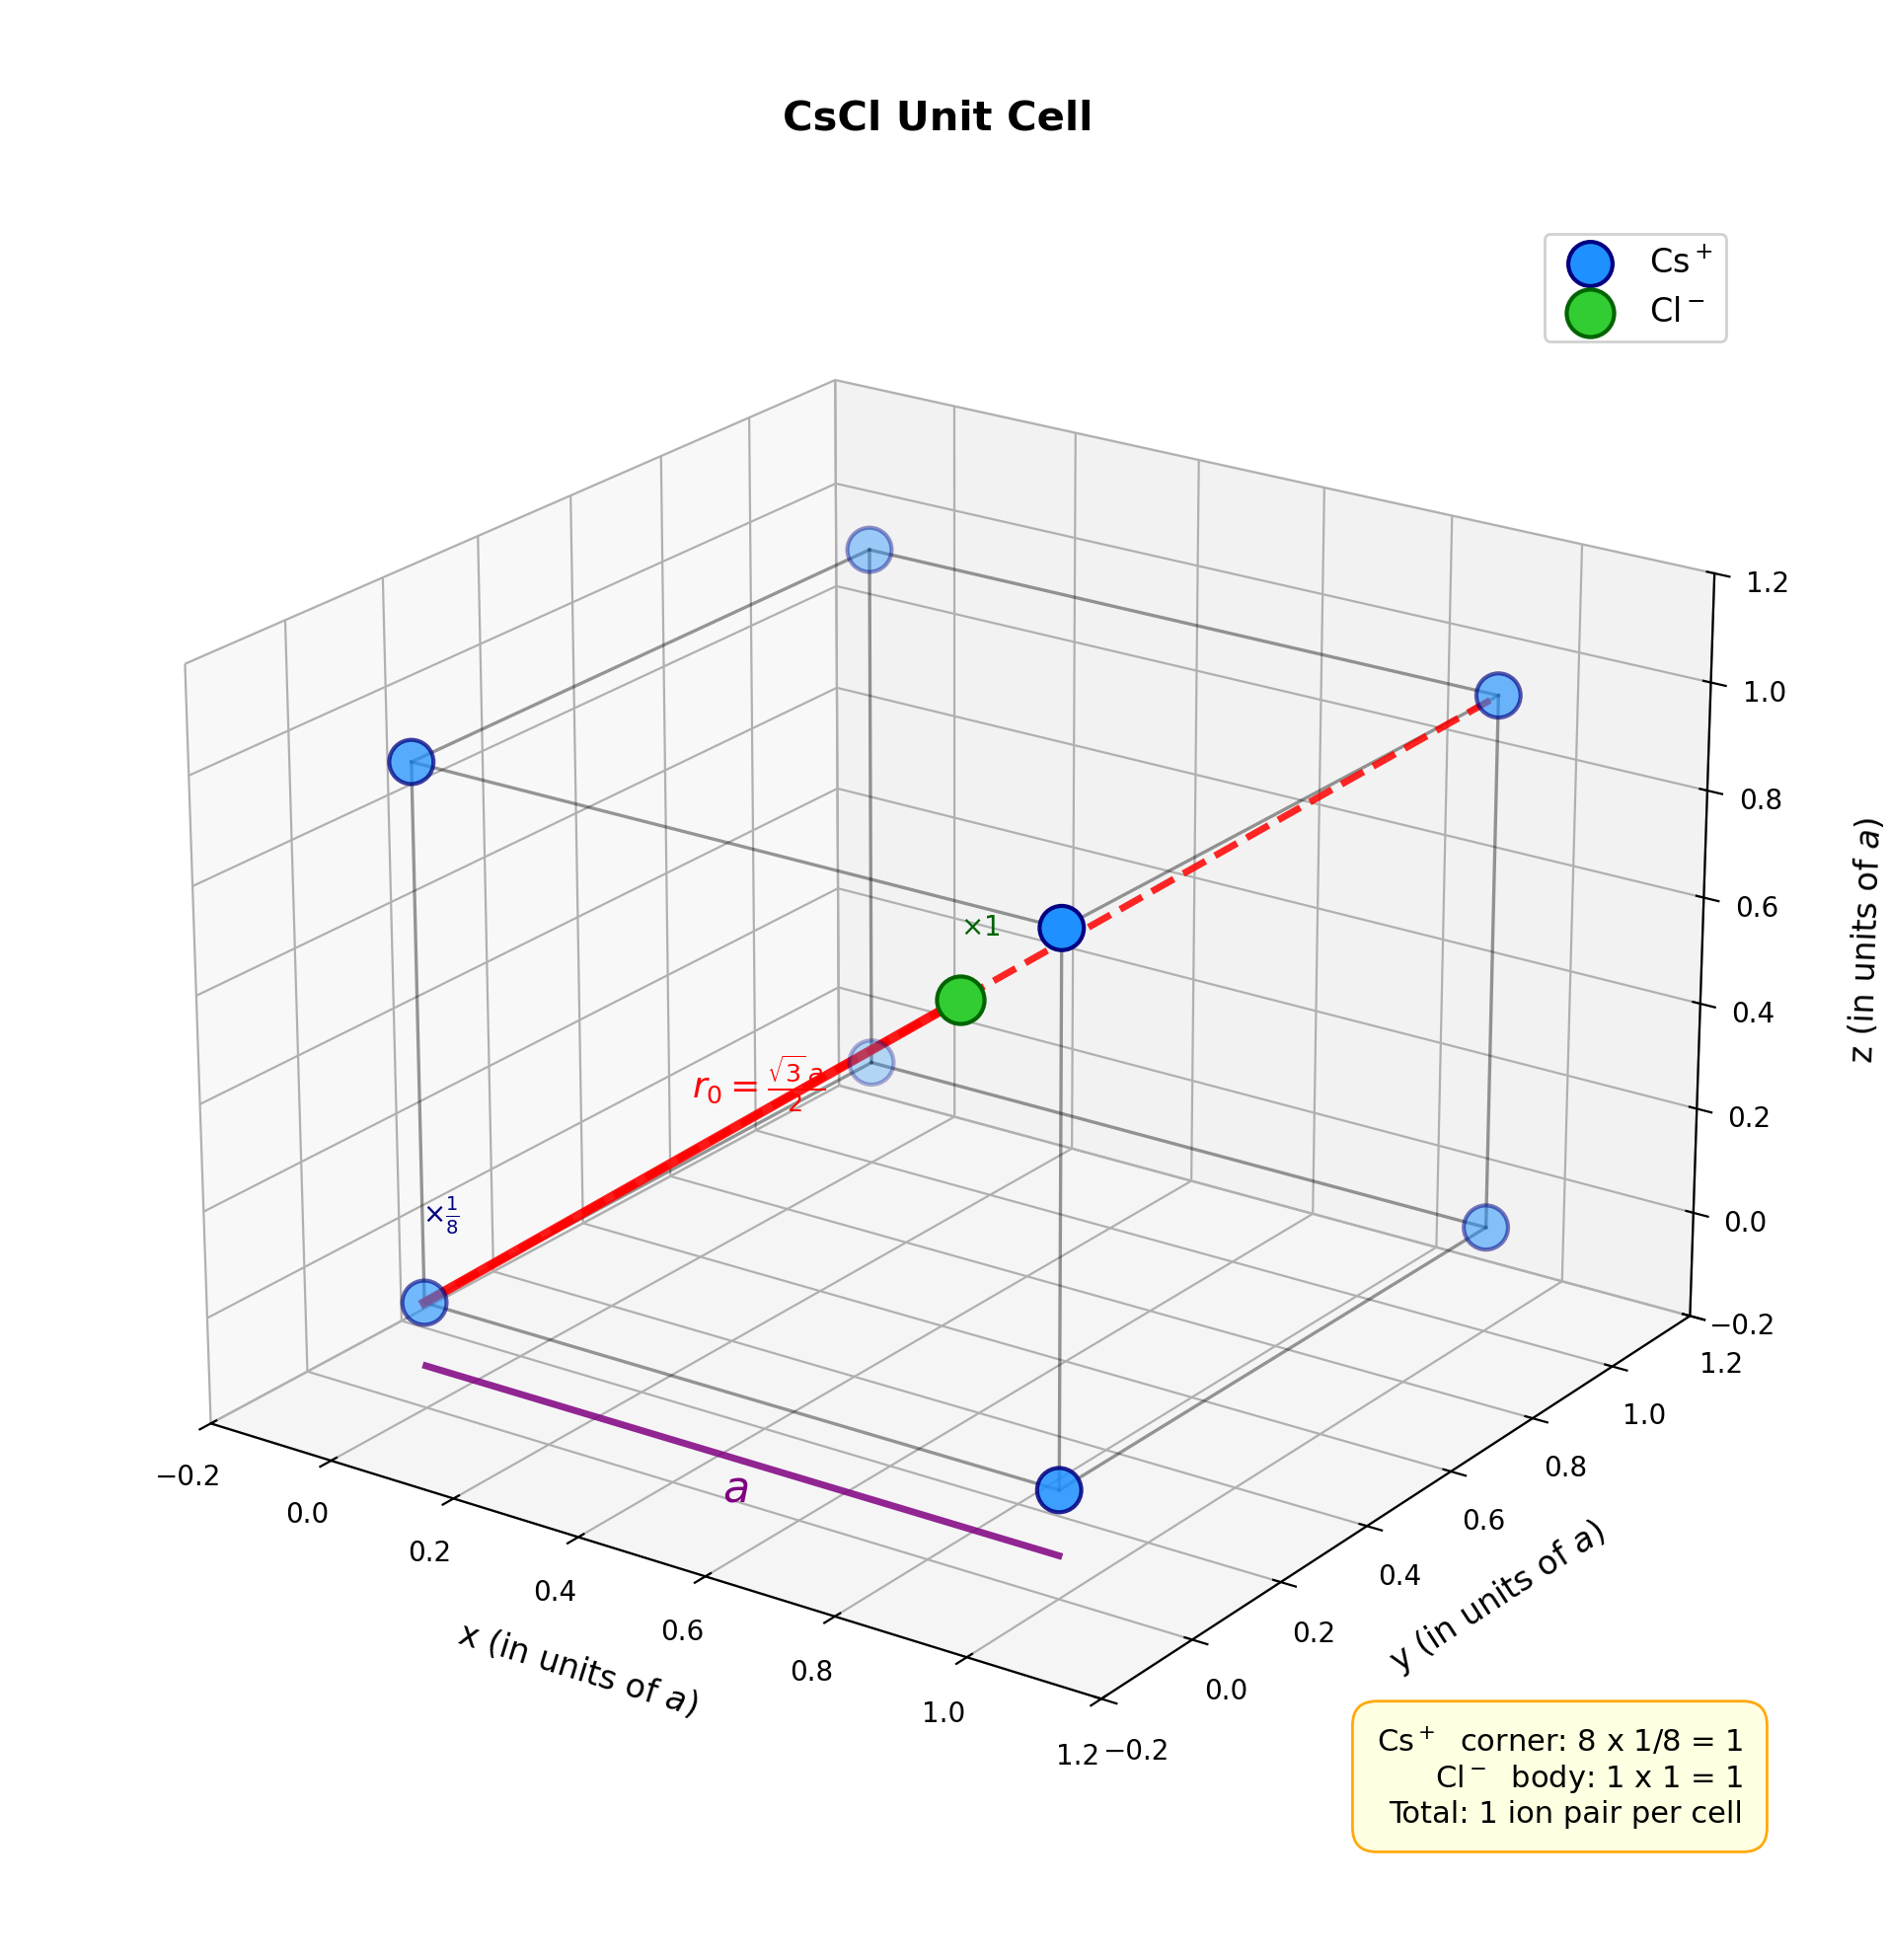
\includegraphics[width=0.78\textwidth]{images/cscl_unit_cell.png}
  \caption{CsCl 晶胞的 3D 示意图。蓝色球为 Cs$^+$（位于立方体 8 个角上），绿色球为 Cl$^-$（位于体心）。红色实线为最近邻间距 $r_0 = \sqrt{3}\,a/2$（体对角线的一半），紫色线段标注晶胞边长 $a$。注意：角上的 Cs$^+$ 被 8 个相邻晶胞共享，每个只计 $1/8$，总计 $8 \times 1/8 = 1$ 个 Cs$^+$；体心 Cl$^-$ 完全属于该晶胞，计 1 个；故每个晶胞恰好含 1 对离子。}
  \label{fig:cscl-unit-cell}
\end{figure}

平衡时体积为
\[
  V_0 = N\alpha r_0^3. \tag{2}
\]

对体积求导得
\[
  \left(\frac{\dd V}{\dd r}\right)_{r_0} = 3N\alpha r_0^2
  \quad\Longrightarrow\quad
  \left(\frac{\dd r}{\dd V}\right)_{r_0} = \frac{1}{3N\alpha r_0^2}. \tag{3}
\]

\subsection{利用平衡条件化简二阶导数}

平衡条件为势能的一阶导数为零：
\[
  \left.\frac{\partial U}{\partial r}\right|_{r_0}
  = N\left[\frac{Me^2}{4\pi\varepsilon_0 r_0^2} - \frac{Z\lambda}{\rho}\,e^{-r_0/\rho}\right] = 0.
\]

由此得到关键关系式：
\[
  \boxed{ e^{-r_0/\rho} = \frac{Me^2\rho}{4\pi\varepsilon_0 Z\lambda r_0^2} }. \tag{*}
\]

\subsubsection{求二阶导数}

\[
  \frac{\partial^2 U}{\partial r^2}
  = N\left[-\frac{2Me^2}{4\pi\varepsilon_0 r^3} + \frac{Z\lambda}{\rho^2}\,e^{-r/\rho}\right].
\]

在 $r = r_0$ 处，代入平衡关系式 $(*)$：
\begin{align*}
  \left.\frac{\partial^2 U}{\partial r^2}\right|_{r_0}
  &= N\left[-\frac{Me^2}{2\pi\varepsilon_0 r_0^3}
       + \frac{1}{\rho^2}\cdot\frac{Me^2\rho}{4\pi\varepsilon_0 r_0^2}\right] \\
  &= \frac{NMe^2}{4\pi\varepsilon_0 r_0^2}\left(-\frac{2}{r_0} + \frac{1}{\rho}\right) \\
  &= \frac{NMe^2}{4\pi\varepsilon_0 r_0^2}\left(\frac{1}{\rho} - \frac{2}{r_0}\right). \tag{4}
\end{align*}

\subsection{计算弹性模量 $K$ 与压缩系数 $B$}

将 (2)、(3)、(4) 代入 (1) 式：
\begin{align*}
  K &= (N\alpha r_0^3)\cdot\left(\frac{1}{3N\alpha r_0^2}\right)^2
      \cdot\frac{NMe^2}{4\pi\varepsilon_0 r_0^2}\left(\frac{1}{\rho} - \frac{2}{r_0}\right) \\
    &= \frac{N\alpha r_0^3}{9N^2\alpha^2 r_0^4}
      \cdot\frac{NMe^2}{4\pi\varepsilon_0 r_0^2}\left(\frac{1}{\rho} - \frac{2}{r_0}\right) \\
    &= \frac{Me^2}{36\pi\varepsilon_0\alpha r_0^3}
      \left(\frac{1}{\rho} - \frac{2}{r_0}\right).
\end{align*}

整理括号内的符号（注意稳定平衡要求 $K>0$，而 $\rho \ll r_0$，故 $\frac{1}{2\rho} > \frac{1}{r_0}$）：
\[
  \frac{1}{\rho} - \frac{2}{r_0} = 2\left(\frac{1}{2\rho} - \frac{1}{r_0}\right).
\]

因此
\[
  K = \frac{Me^2}{18\pi\varepsilon_0\alpha r_0^3}
      \left(\frac{1}{2\rho} - \frac{1}{r_0}\right) > 0.
\]

利用 $V_0 = N\alpha r_0^3$，可把 $\alpha r_0^3$ 替换为 $V_0/N$：
\[
  K = \frac{NMe^2}{18\pi\varepsilon_0 V_0}
      \left(\frac{1}{2\rho} - \frac{1}{r_0}\right).
\]

取倒数得压缩系数：
\[
  \boxed{ B = \frac{1}{K}
         = \frac{18\pi\varepsilon_0 V_0}{NMe^2}
           \left(\frac{1}{r_0} - \frac{1}{2\rho}\right)^{-1} }.
\]

\begin{insightbox}{考场手绘晶体结构的技巧——从 2D 正视图入手}
\textbf{最大误区}：一上来就画 3D 透视图，结果框架歪歪扭扭，离子互相遮挡。\textbf{正确做法}：先画\textbf{正视图}（或俯视图），需要时再补一个简单的轴测图。

\textbf{NaCl 结构——三步法}（对照图 \ref{fig:nacl-unit-cell}）：
\begin{enumerate}[nosep]
  \item \textbf{画正方形}：这就是晶胞的一个面，边长标 $a$；
  \item \textbf{角和面心画圈}（Na$^+$）：四个角 + 中心一个圈；
  \item \textbf{四条边的中点画叉}（Cl$^-$）：搞定。
\end{enumerate}

\textbf{如果需要 3D 效果}——斜二测画法（对照图 \ref{fig:nacl-unit-cell}）：
\begin{enumerate}[nosep]
  \item 先画前面的正方形（正常画）；
  \item 从四个角向右上方拉三条\textbf{平行线}（角度约 $45^\circ$，长度约为边长的一半）；
  \item 连接后端点，形成后面的正方形；
  \item 按同样的规则填圈和叉。
\end{enumerate}

\textbf{CsCl 结构}：
\begin{enumerate}[nosep]
  \item 画一个简单立方体；
  \item 八个角画圆圈 $\circ$（Cs$^+$）；
  \item 正中央画叉 $\times$（Cl$^-$）。
\end{enumerate}

\textbf{核心原则}：
\begin{itemize}[nosep]
  \item \textbf{不要画实心球}——会互相遮挡，看不出内部结构；
  \item \textbf{用不同符号}（圈/叉/点）区分两种离子，比用颜色更可靠；
  \item \textbf{先画框架，再填离子}——框架是参照系，没有框架离子就飘在空中；
  \item \textbf{2D 正视图足够应付大多数考题}——只有明确要求画 3D 时才画轴测图。
\end{itemize}
\end{insightbox}

\begin{insightbox}{晶体结构手绘：元胞、密铺、WS 原胞的实战策略}

\textbf{一、元胞画法——2$\times$2 框选法}

画单个晶胞时，角上的原子只露 1/8、棱上的只露 1/4，看起来支离破碎。\textbf{解决方法是先画 2$\times$2（或 2$\times$2$\times$2）阵列，再框选一个晶胞}：
\begin{enumerate}[nosep]
  \item \textbf{画格点阵列}：比如简单立方，先画 $2\times 2$ 的四个正方形（或 $2\times 2\times 2$ 的立方体阵列）；
  \item \textbf{填完整原子}：所有原子都用完整符号（圈/叉）画出，不要画"缺角"的原子；
  \item \textbf{粗线框选一个晶胞}：用粗线或阴影标出其中一个元胞的范围；
  \item \textbf{在框内标注分摊}：框内的原子按位置（角、棱、面、体心）标注权重，框外的原子不用管。
\end{enumerate}

\textbf{为什么有效}：在 $2\times 2$ 阵列中，内部原子是"完整"的，只有框边界上的原子需要想分摊问题。框出一个晶胞后，你可以清楚地看到它包含哪些原子、各占多少权重。\textbf{画多了不是错，画少了看不清才是错}。

\vspace{0.5em}
\textbf{二、密铺（Close Packing）——空隙定位法}

密堆结构考的是\textbf{层间几何关系}，不是画球。A/B/C 三层容易乱，改用\textbf{空隙定位}：
\begin{enumerate}[nosep]
  \item \textbf{A 层}：画 7 个紧密相切的圆呈六方蜂窝（1 中心 + 6 近邻），标为 A 层；
  \item \textbf{B 层位置}：每 3 个相邻 A 层原子围成一个正三角形凹陷，B 层原子就坐在这个凹陷正上方。在俯视图中，用一个小圆点（或不同颜色/线型）标在三角形中心，代表 B 层；
  \item \textbf{C 层位置}：C 层也坐在 A 层的凹陷上，但\textbf{与 B 层错位}——B 层占了一部分凹陷，C 层占另一部分。从俯视图看，若 A 层格点构成六角网格，B 层在 "A 层三角形中心"，C 层在 "A 层另一种三角形中心"（两种三角形交替排列）。
\end{enumerate}

\textbf{判断 fcc/hcp 不看三层，看重复周期}：
\begin{itemize}[nosep]
  \item \textbf{hcp}：第 3 层回到 A 层位置 → 周期 AB，六方晶胞 $c/a = \sqrt{8/3} \approx 1.633$；
  \item \textbf{fcc}：第 3 层到 C 层位置，第 4 层才回 A → 周期 ABC，密堆面是 \{111\}。
\end{itemize}

\textbf{关键}：配位数都是 12，空隙都是四面体空隙和八面体空隙。考题问"哪种堆积更密"——一样密；问"哪种对称性更高"——fcc（立方对称）。

\vspace{0.5em}
\textbf{三、Wigner-Seitz 原胞——考试中实际考什么}

WS 原胞的定义是"以一个格点为中心，到最近邻的垂直平分面围成的区域"。考试中的实际考法有三种：

\begin{enumerate}[nosep]
  \item \textbf{考定义/性质}（最常见）：WS 原胞与第一布里渊区的关系、WS 原胞体积等于原胞体积。这种题\textbf{不需要画图}，记概念即可；
  \item \textbf{考 2D 格子}（偶尔）：比如正方格子或六角格子。画法是：标出中心格点和 4 个（正方）或 6 个（六角）最近邻 → 连中心到最近邻 → 在各连线中点作\textbf{垂直平分线} → 围成的多边形就是 WS 原胞；
  \item \textbf{考 3D 拓扑}（选择题/填空题）：sc $\to$ 立方体（6 面），bcc $\to$ 截角八面体（14 面），fcc $\to$ 菱形十二面体（12 面）。\textbf{记面数和形状名称}即可。
\end{enumerate}

\textbf{"画晶面"是什么意思}：就是画一个二维切片。比如立方晶系的 $(001)$ 面，就是垂直于 $z$ 轴、$z=0$ 的平面。在这个平面上，格点排列成一个正方形网格，你就可以像画 2D 正方格子一样画 WS 截面了。

\textbf{为什么不教 3D 手绘}：因为考试中\textbf{几乎不考 3D WS 原胞的手绘图}。如果真的遇到，画一个 2D 截面并标注"此为 WS 原胞在某晶面的截面"，比硬画一个歪歪扭扭的截角八面体得分更高。

\begin{center}
\renewcommand{\arraystretch}{1.4}
\begin{tabular}{|l|c|l|l|}
\hline
\textbf{格子} & \textbf{最近邻数} & \textbf{WS 形状} & \textbf{考试应对} \\
\hline
sc & 6 & 立方体 & 就是原胞本身 \\
bcc & 8 & 截角八面体 & 记"14 面体，6 正方 + 8 六边" \\
fcc & 12 & 菱形十二面体 & 记"12 个全等菱形面" \\
\hline
\end{tabular}
\end{center}

\vspace{0.5em}
\textbf{四、错位双原子格子——子晶格平移法}

NaCl、CsCl、ZnS（闪锌矿）都是\textbf{双原子复式格子}，可以看成两套\textbf{同型布拉维格子}沿某方向平移套构而成：
\begin{itemize}[nosep]
  \item \textbf{NaCl}：Cl$^-$ 形成 fcc，Na$^+$ 的 fcc 沿 $[100]$ 方向平移 $a/2$（即 Na$^+$ 位于 Cl$^-$ 的棱心和体心位置）；
  \item \textbf{CsCl}：两套简单立方沿体对角线平移 $\sqrt{3}\,a/2$（即体心位置）；
  \item \textbf{闪锌矿 ZnS}：与金刚石结构同型，两套 fcc 沿体对角线平移 $\sqrt{3}\,a/4$。
\end{itemize}

\textbf{手绘策略}（配合 2$\times$2 框选法）：
\begin{enumerate}[nosep]
  \item 先画其中一套\textbf{完整的 2$\times$2 格点阵列}（比如用圆圈表示 Cl$^-$）；
  \item 框出一个晶胞，在框内的平移后位置用\textbf{另一种符号}（叉或实心点）标记第二种原子；
  \item 框外的第二种原子不画，只保留第一种原子的阵列作为\textbf{背景参照系}。
\end{enumerate}

\textbf{关键认知}：双原子格子的"错位"不是混乱，而是\textbf{严格的平移对称操作}。只要记住"fcc + fcc 平移 $a/2$ = NaCl"、"sc + sc 平移体对角线一半 = CsCl"，就不用死记每个离子的坐标。
\end{insightbox}

\begin{insightbox}{与 NaCl 结合能题的对比}
\begin{center}
\renewcommand{\arraystretch}{1.5}
\begin{tabular}{|l|c|c|}
\hline
\textbf{题目} & \textbf{已知} & \textbf{求} \\
\hline
NaCl 结合能 & 比重 $D$、弹性模量 $K$ & 结合能 $U_0$ \\
压缩系数 & 势函数 $U(r)$ & 压缩系数 $B = 1/K$ \\
\hline
\end{tabular}
\end{center}

两道题的\textbf{共同核心}：
\begin{enumerate}[nosep]
  \item 都用到 $V = N\alpha r^3$ 的体积-间距关系；
  \item 都用到平衡条件化简二阶导数；
  \item 最终都出现 $\left(\dfrac{1}{r_0} - \dfrac{1}{2\rho}\right)$ 形式的结构因子。
\end{enumerate}

区别仅在于 NaCl 结合能题用\textbf{幂律排斥} $B/r^n$，本题用\textbf{指数排斥} $Z\lambda e^{-r/\rho}$。指数形式的化简更优雅——平衡条件直接给出 $e^{-r_0/\rho}$ 的显式表达式，避免了幂律形式需要先求 $n$ 再代入的繁琐步骤。
\end{insightbox}
